% Created 2018-01-12 vie 00:19
% Intended LaTeX compiler: pdflatex
\documentclass[xcolor={usenames,svgnames,dvipsnames}]{beamer}
\usepackage[utf8]{inputenc}
\usepackage[T1]{fontenc}
\usepackage{graphicx}
\usepackage{grffile}
\usepackage{longtable}
\usepackage{wrapfig}
\usepackage{rotating}
\usepackage[normalem]{ulem}
\usepackage{amsmath}
\usepackage{textcomp}
\usepackage{amssymb}
\usepackage{capt-of}
\usepackage{hyperref}
\usepackage{color}
\usepackage{listings}
\usepackage{mathpazo}
\usepackage{gensymb}
\usepackage{amsmath}
\usepackage{chemarr}%flechas para reacciones químicas (SFER.tex)
\bibliographystyle{plain}
\AtBeginSubsection[]{\begin{frame}[plain]\tableofcontents[currentsubsection,sectionstyle=show/shaded,subsectionstyle=show/shaded/hide]\end{frame}}
\AtBeginSection[]{\begin{frame}[plain]\tableofcontents[currentsection,hideallsubsections]\end{frame}}
\usepackage[emulate=units]{siunitx}
\sisetup{fraction=nice, decimalsymbol=comma, retain-unity-mantissa = false}
\newunit{\wattpeak}{Wp}
\newunit{\watthour}{Wh}
\newunit{\amperehour}{Ah}
\hypersetup{colorlinks=true, linkcolor=Blue, urlcolor=Blue}
\renewcommand{\thefootnote}{\fnsymbol{footnote}}
\setbeamercolor{alerted text}{fg=blue!50!black} \setbeamerfont{alerted text}{series=\bfseries}
\usetheme[hideothersubsections]{Goettingen}
\usecolortheme{rose}
\usefonttheme{serif}
\author{Oscar Perpiñán Lamigueiro \\ \url{http://oscarperpinan.github.io}}
\date{}
\title{Sistemas Fotovoltaicos Autónomos}
\subtitle{Conceptos Generales y Componentes}
\hypersetup{
 pdfauthor={Oscar Perpiñán Lamigueiro \\ \url{http://oscarperpinan.github.io}},
 pdftitle={Sistemas Fotovoltaicos Autónomos},
 pdfkeywords={},
 pdfsubject={},
 pdfcreator={Emacs 25.2.2 (Org mode 9.1.6)}, 
 pdflang={Spanish}}
\begin{document}

\maketitle

\section{Conceptos Generales}
\label{sec:orgba2c4d4}

\begin{frame}[label={sec:orge1db5ef}]{Definición de un Sistema Autónomo}
Un sistema fotovoltaico autónomo (SFA) produce energía eléctrica para \alert{satisfacer el consumo de cargas eléctricas no conectadas a la red}, \alert{empleando un sistema de acumulación energético} para hacer frente a los períodos en los que la generación es inferior al consumo.
\end{frame}

\begin{frame}[label={sec:org0356d8c}]{Configuracion SHS}
\begin{center}
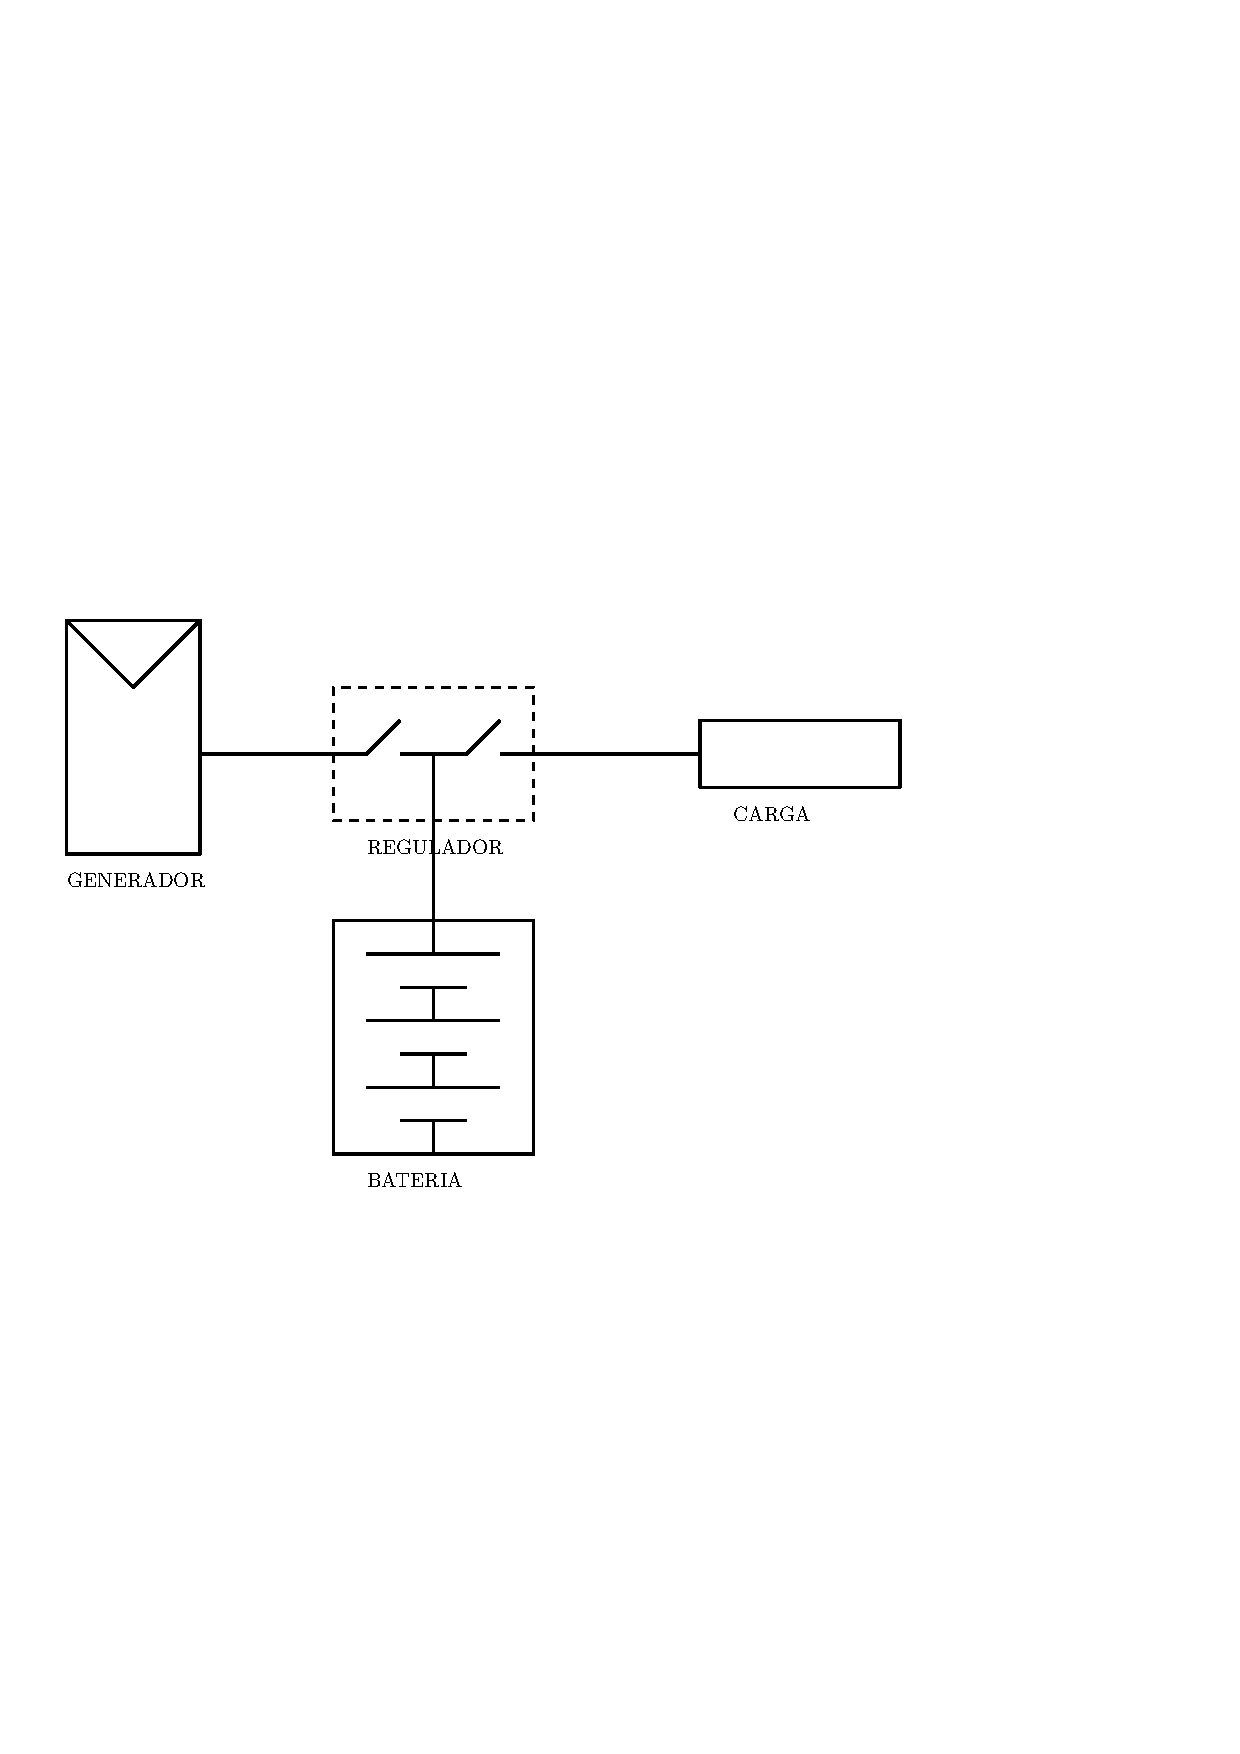
\includegraphics[width=.9\linewidth]{../figs/DiagramaUnifilarER_DC.pdf}
\end{center}
\end{frame}

\begin{frame}[label={sec:org2dfa709}]{Configuración AC}
\begin{center}
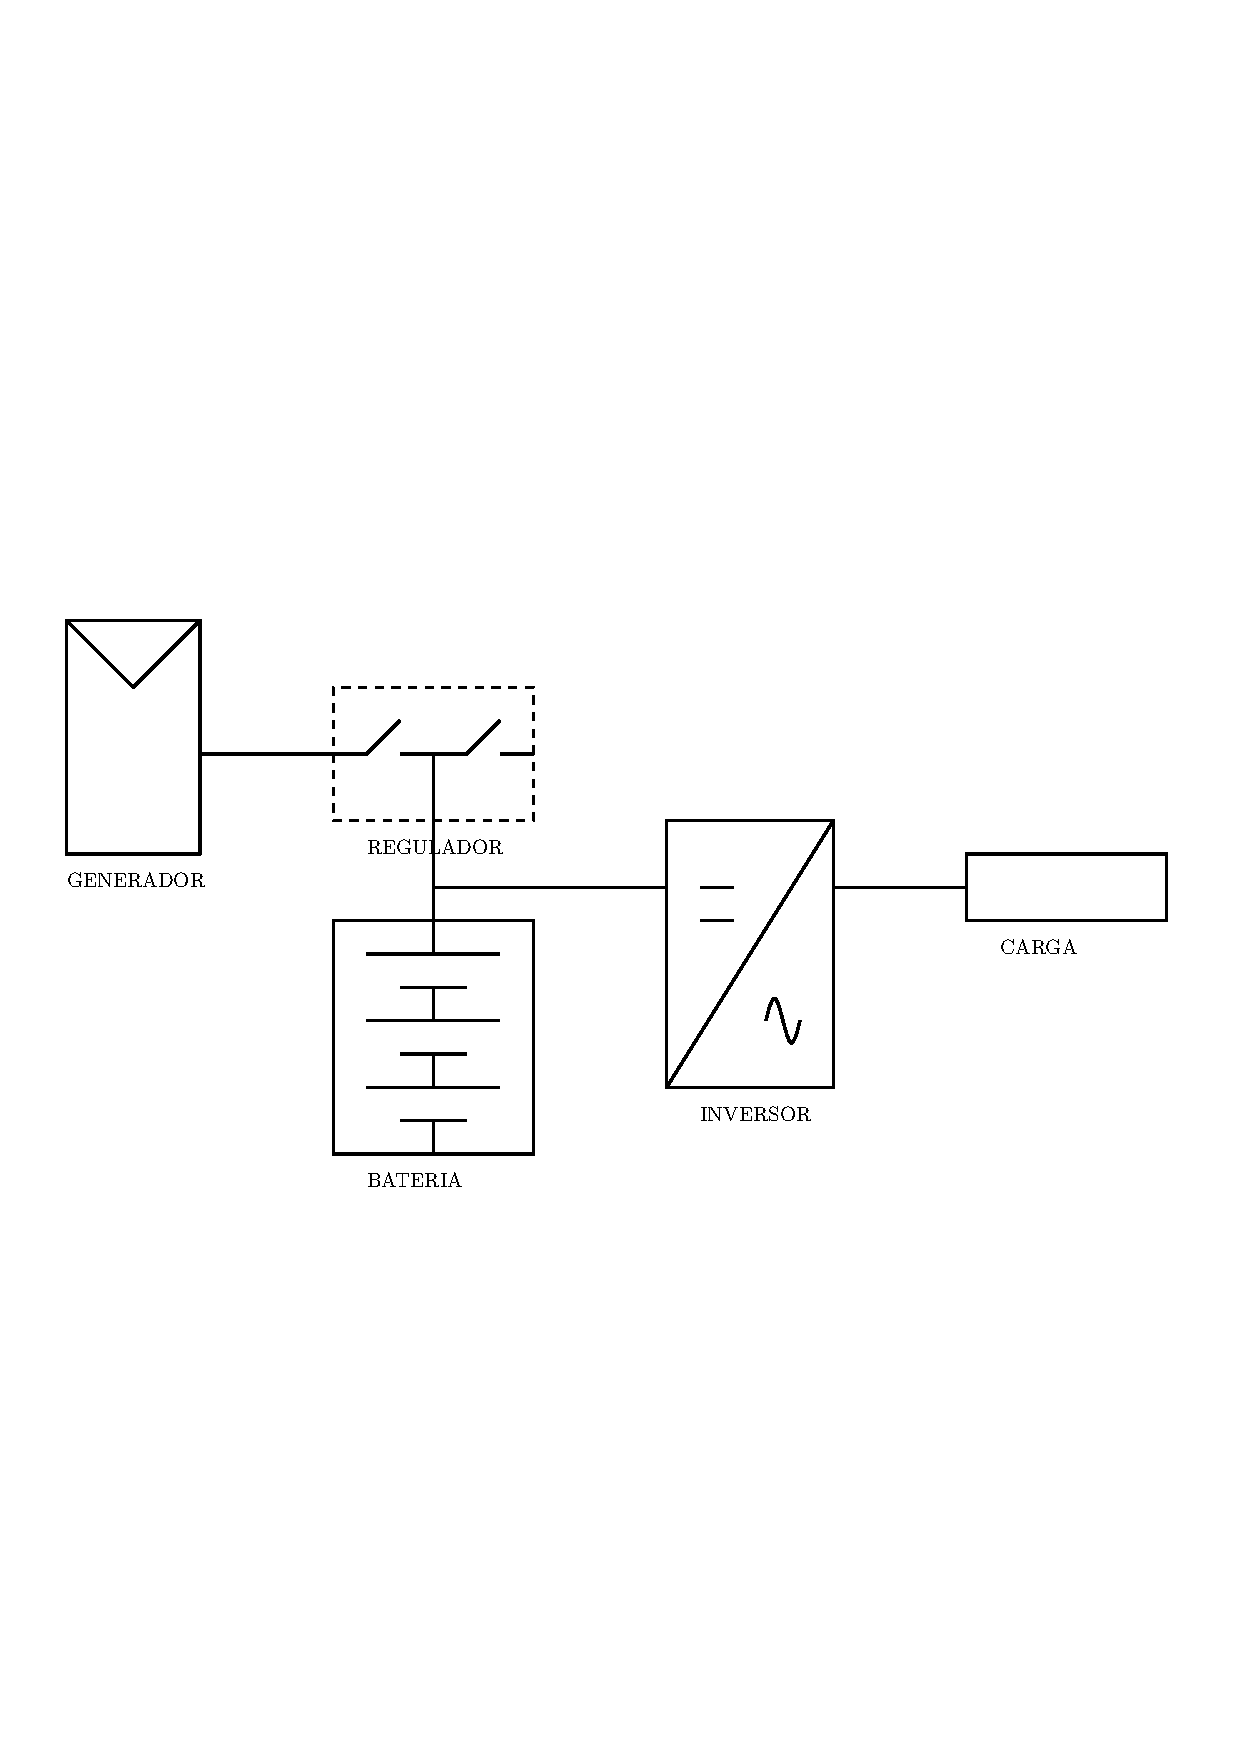
\includegraphics[width=.9\linewidth]{../figs/DiagramaUnifilarER_AC.pdf}
\end{center}
\end{frame}

\begin{frame}[label={sec:org677bc3c}]{Configuración DC+AC}
\begin{center}
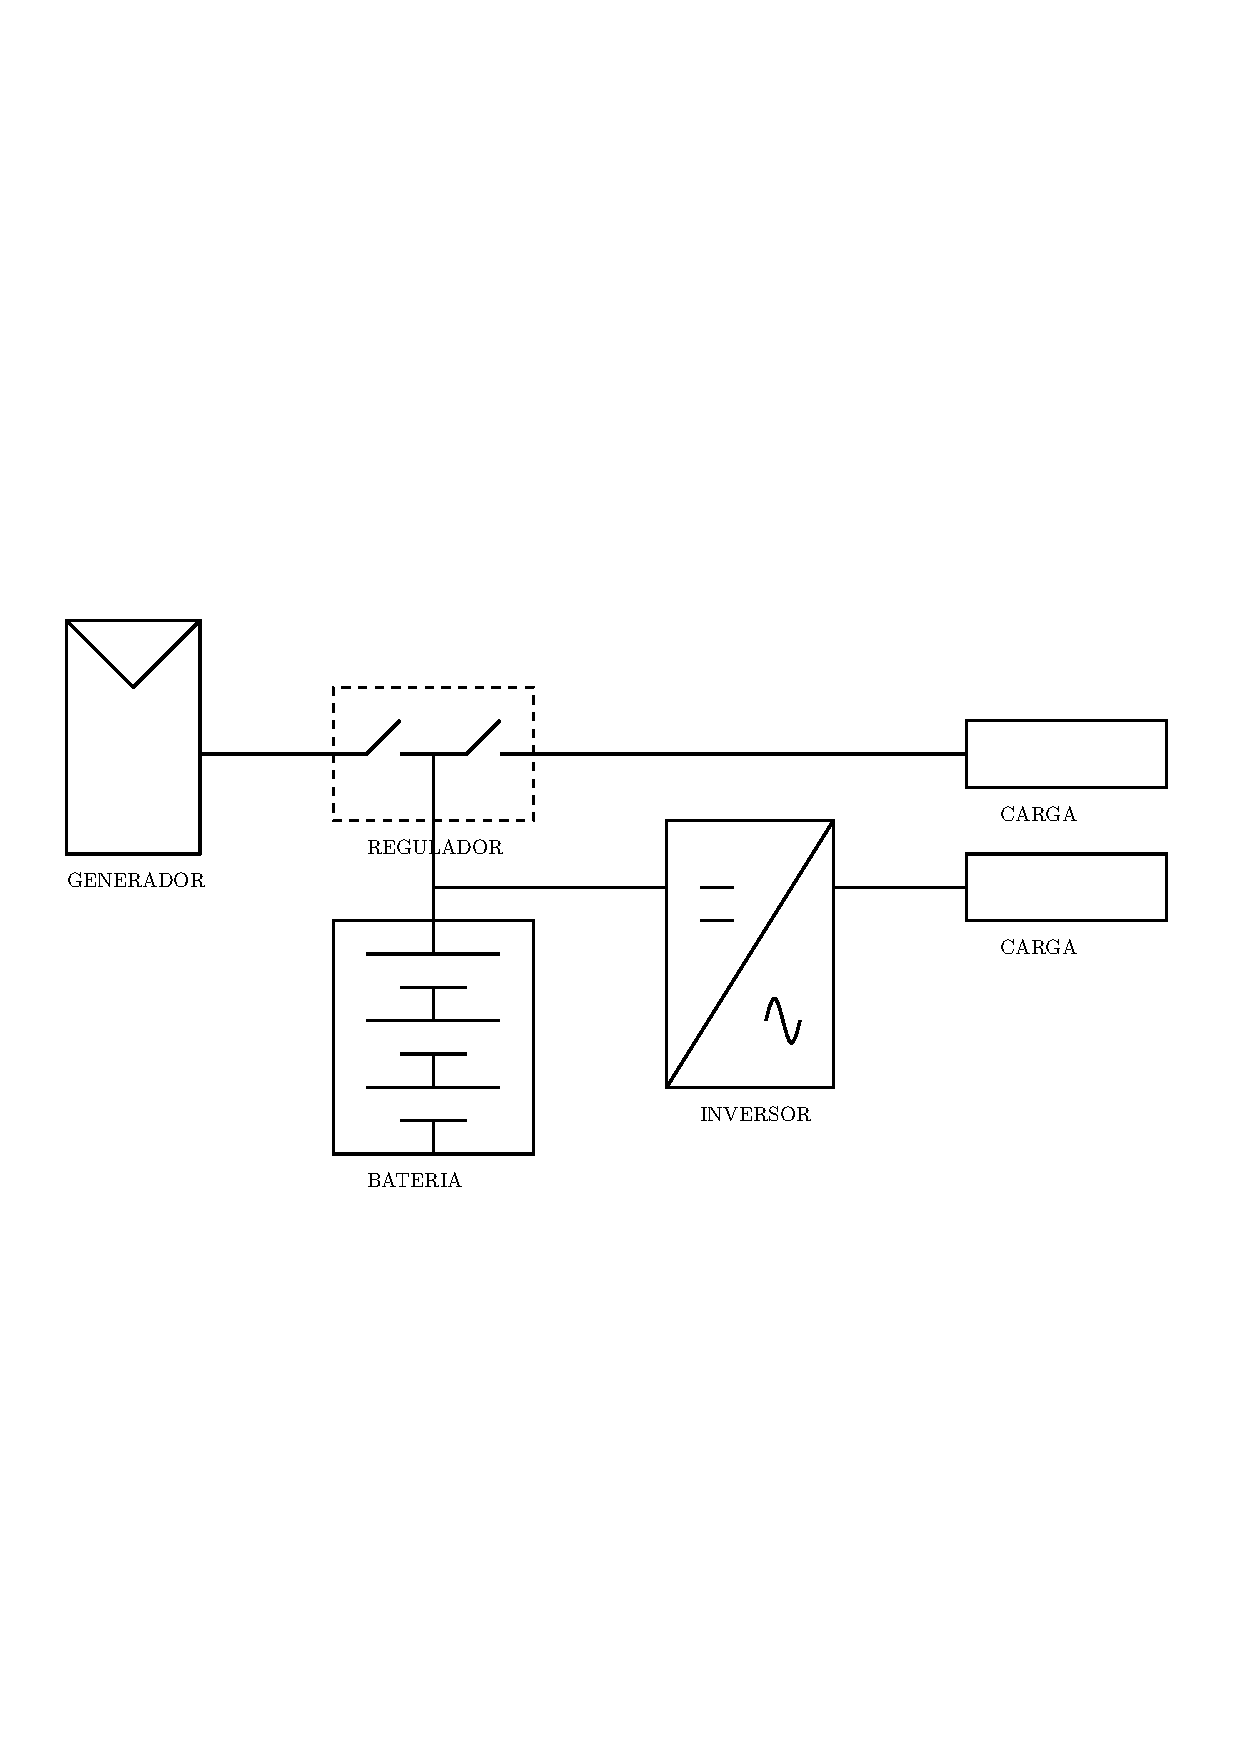
\includegraphics[width=.9\linewidth]{../figs/DiagramaUnifilarER_AC_DC.pdf}
\end{center}
\end{frame}

\begin{frame}[label={sec:org6c43b9a}]{Sistema Híbrido}
\begin{center}
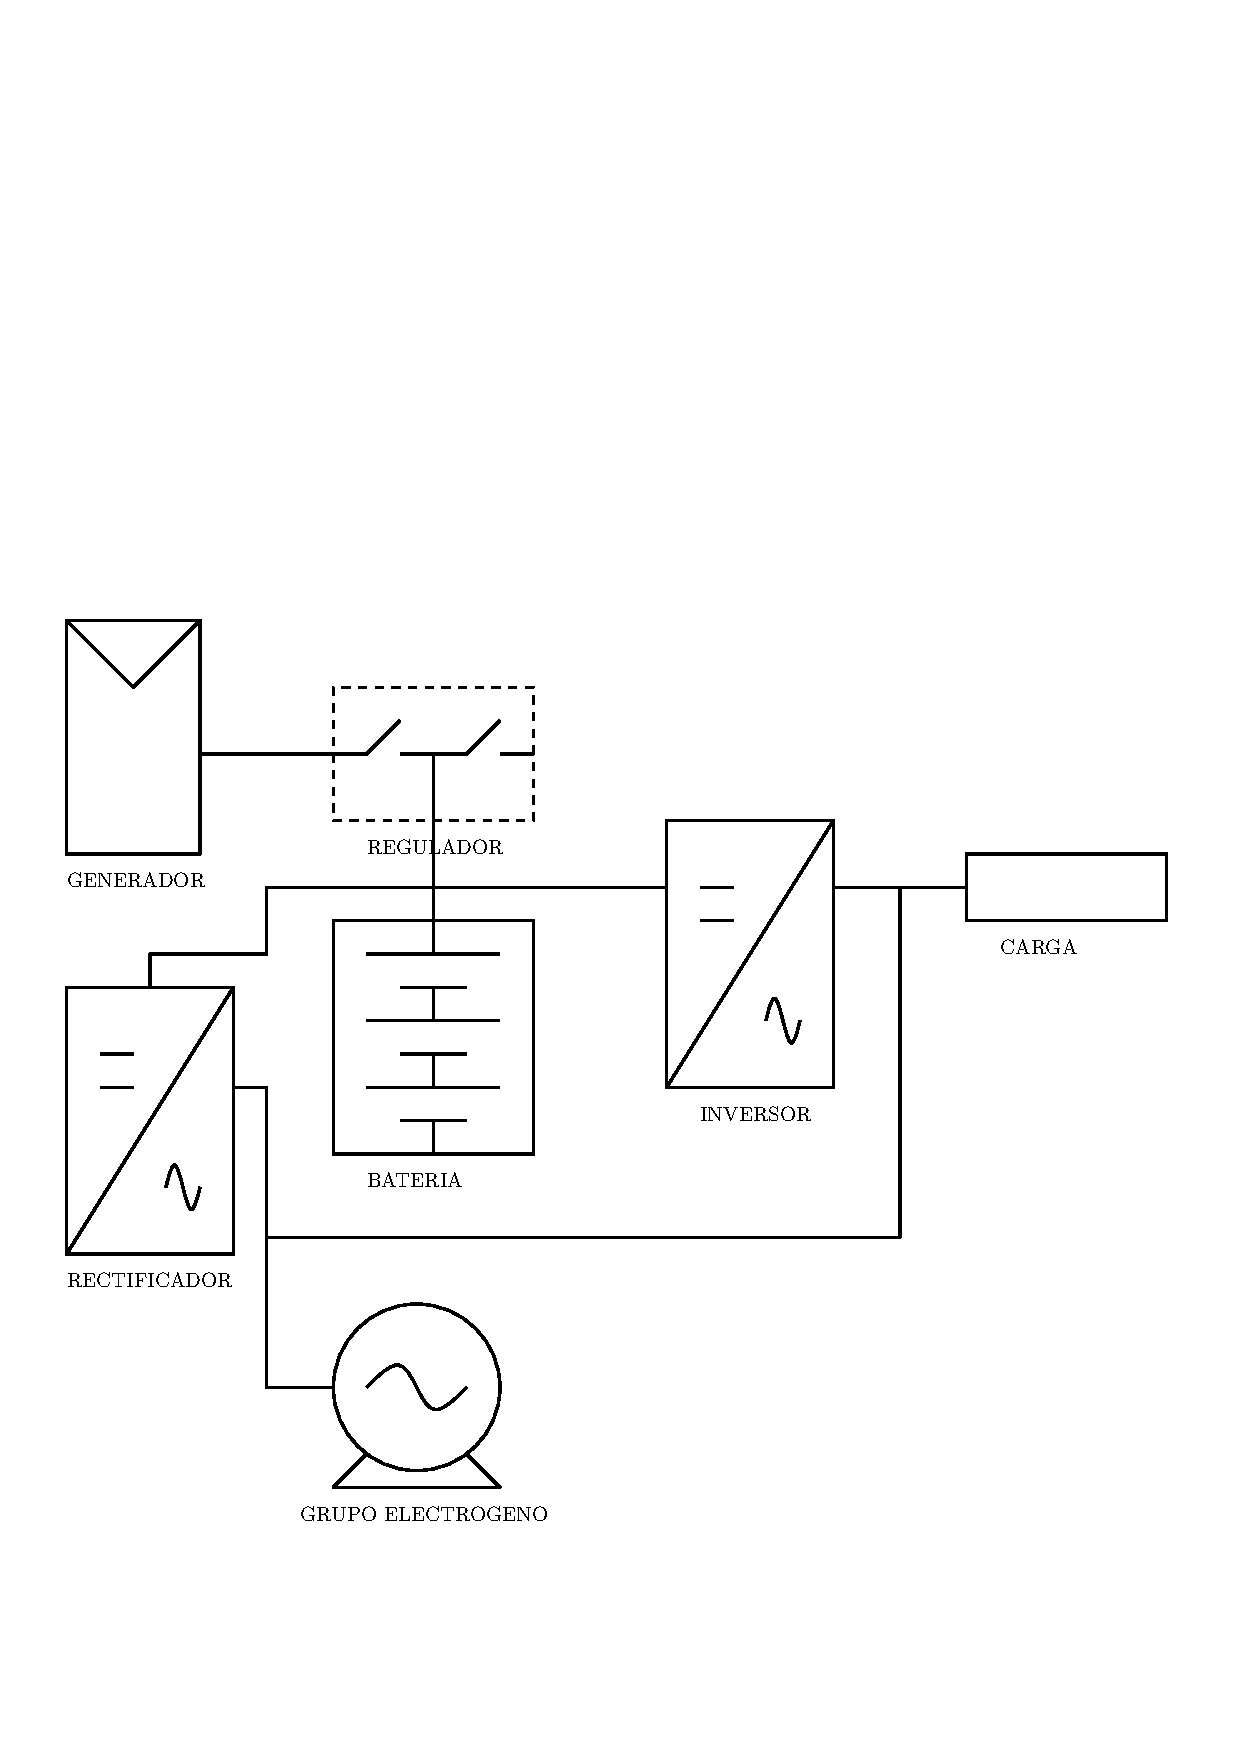
\includegraphics[width=.9\linewidth]{../figs/DiagramaUnifilarER_Hibrido.pdf}
\end{center}
\end{frame}

\section{Acumulador Electroquímico}
\label{sec:org0856b40}

\subsection{Definiciones}
\label{sec:orgeba8696}

\begin{frame}[label={sec:org486091f}]{Acumulador electroquímico}
Un acumulador electroquímico es una bateria secundaria o recargable, capaz de almacenar energía eléctrica mediante una transformación en energía electroquímica. Sus principales funciones son:

\begin{itemize}
\item \alert{Autonomía}: satisface los requerimientos de consumo en cualquier momento, independientemente de la generación.

\item \alert{Suministro de picos de intensidad}: cuando es necesario, puede suministrar valores de intensidad superiores a los que proporciona el generador FV.

\item \alert{Estabilización del voltaje}: evita fluctuaciones dañinas para los equipos de consumo.
\end{itemize}
\end{frame}

\begin{frame}[label={sec:orgd67c29e}]{Definiciones}
\begin{description}
\item[{Capacidad nominal (\(C_{nom}\))}] es la carga eléctrica que puede ser extraída de una batería hasta llegar a la descarga total.

\item[{Régimen de carga/descarga}] es la corriente aplicada a una batería para restablecer/extraer la capacidad nominal. Normalmente se presenta como un ratio entre la capacidad nominal y la corriente.

\item[{Estado de carga (SoC)}] de una batería es la capacidad de una batería parcialmente cargada, dividida por su capacidad nominal. Por tanto siempre será \(0<SoC<1\).
\end{description}
\end{frame}

\begin{frame}[label={sec:org5e60268}]{Definiciones}
\begin{description}
\item[{Profundidad de descarga (PD)}] es el complemento del estado de carga.

\item[{Tensión de corte:}] es la tensión a la que finaliza la descarga de la batería. Depende del régimen de descarga y del tipo de batería.  Determina la profundidad de descarga máxima, \(PD_{max}\), y por tanto, la capacidad útil, \(C_{U}\), siendo $$C_{U}=PD_{max}\cdot C_{nom}$$
\end{description}
\end{frame}

\begin{frame}[label={sec:orge45fbea}]{Definiciones}
\begin{description}
\item[{Eficiencia farádica}] es el ratio entre la carga extraída durante la descarga y la carga requerida para restablecer el estado inicial.

\item[{Eficiencia energética}] es el ratio entre la energía extraída durante la descarga y la energía requerida para restablecer el estado inicial.
\end{description}
\end{frame}

\subsection{Principios de funcionamiento}
\label{sec:org111cbca}

\begin{frame}[label={sec:org1cdd909}]{Composición}
Una batería de ácido-plomo se compone de:

\begin{itemize}
\item Un \alert{ánodo o electrodo positivo} con PbO\(_{\text{2}}\)

\item Un \alert{cátodo o electrodo negativo} con Pb.

\item \alert{Electrolito} a base de \(H_{2}SO_{4}\) diluido en agua.
\end{itemize}

\begin{center}
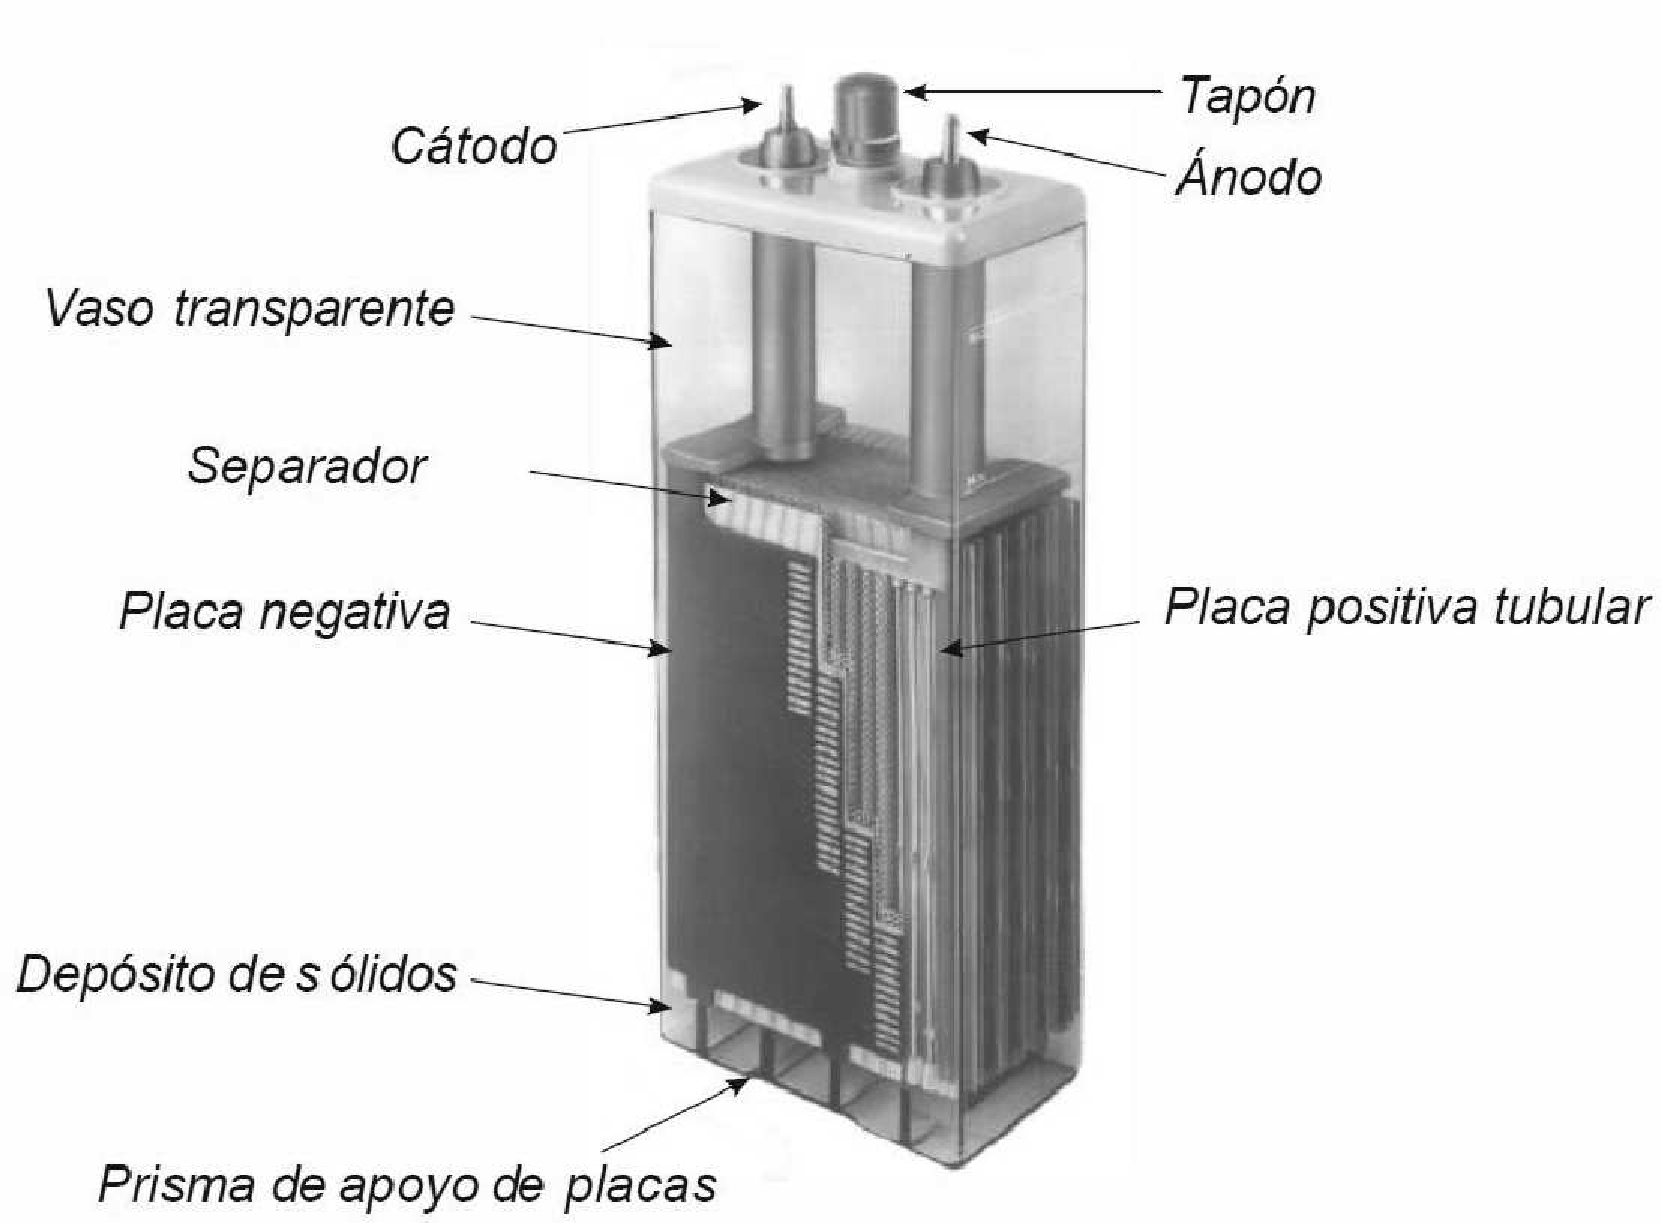
\includegraphics[width=.9\linewidth]{../figs/AcumuladorBN.pdf}
\end{center}
\end{frame}



\begin{frame}[label={sec:org62b453f}]{Reacción Química REDOX}
\begin{itemize}
\item Ánodo (+):
\end{itemize}

\[
\mathrm{PbO_{2}+SO_{4}^{2-}+H^{+}+2e^{-}
\xrightleftharpoons[\text{carga}]{\text{descarga}}
  PbSO_{4}+2H_{2}O}
\]

\begin{itemize}
\item Cátodo (-):
\end{itemize}
\[
\mathrm{Pb+SO_{4}^{2-}
\xrightleftharpoons[\text{carga}]{\text{descarga}}
PbSO_{4}+2e^{-}}
\]

\begin{itemize}
\item Global:
\end{itemize}
\[
\mathrm{Pb+PbO_{2}+2H_{2}SO_{4}
\xrightleftharpoons[\text{carga}]{\text{descarga}}
2PbSO_{4}+2H_{2}O}
\]
\end{frame}


\begin{frame}[label={sec:orgf54fabe}]{Descarga}
\[
\mathrm{Pb+PbO_{2}+2H_{2}SO_{4}} \rightarrow \mathrm{2PbSO_{4}+2H_{2}O}
\]

\begin{itemize}
\item \alert{Consumo de electrolito} (disminuye su densidad)

\item \alert{Cambios de volumen} de los materiales activos.

\item \alert{Descargas repetidas} producen \alert{pérdida de material activo} y degradación de las placas.

\item Si la descarga es muy rápida y la bateria permanece descarga largo tiempo, el sulfato cristaliza y no es recuperable (\alert{sulfatación}).
\end{itemize}
\end{frame}

\begin{frame}[label={sec:orge076ed2}]{Carga}
\[
\mathrm{2PbSO_{4}+2H_{2}O} \rightarrow \mathrm{Pb+PbO_{2}+2H_{2}SO_{4}} 
\]

\begin{itemize}
\item Con largos períodos en estados parciales de carga, el ácido se concentra en el fondo por gravedad (\alert{estratificación})

\begin{itemize}
\item Las reacciones no se producen de igual forma en toda la extensión de las placas, lo que realimenta el proceso.

\item Puede reducirse mediante un \alert{gaseo controlado}.
\end{itemize}

\item Al terminar el proceso de carga se produce la electrolisis del agua, con liberación de oxigeno e hidrógeno (\alert{gaseo}):

\begin{itemize}
\item Pérdida de agua del electrolito (hay que reponerla)

\item Homogeneización del electrolito por agitación (reduce la estratificación)
\end{itemize}
\end{itemize}
\end{frame}

\subsection{Modelo eléctrico}
\label{sec:org5812d40}
\begin{frame}[label={sec:orgcc2e6c2}]{Fuente de tensión}
\begin{itemize}
\item Una batería de ácido-plomo puede ser modelada como una fuente de tensión, \(V_{BI}\), en serie con una resistencia, \(R_{BI}\).
\end{itemize}

\begin{center}
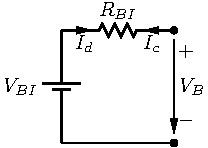
\includegraphics[width=.9\linewidth]{../figs/Bateria.pdf}
\end{center}
\end{frame}

\begin{frame}[label={sec:orge99417d}]{Densidad del electrolito y Tensión en Abierto}
\begin{block}{La medida de la tensión en circuito abierto de la batería es un método común para estimar el estado de carga de una batería.}
\begin{itemize}
\item \(V_{BI}=\rho_{e}+0.84\)

\item Baterías cargadas:

\begin{itemize}
\item \(\SI{1.2}{\gram\per\cm\cubed} \leq \rho_{e}  \leq \SI{1.28}{\gram\per\cm\cubed}\).
\item \(\SI{2.04}{\volt} \leq V_{BI} \leq \SI{2.12}{\volt}\).
\end{itemize}
\item \alert{Hay que corregir con la temperatura}
\end{itemize}
\end{block}
\end{frame}

\begin{frame}[label={sec:org9c2493c}]{Evolución de la tensión durante un proceso de descarga}
\begin{center}
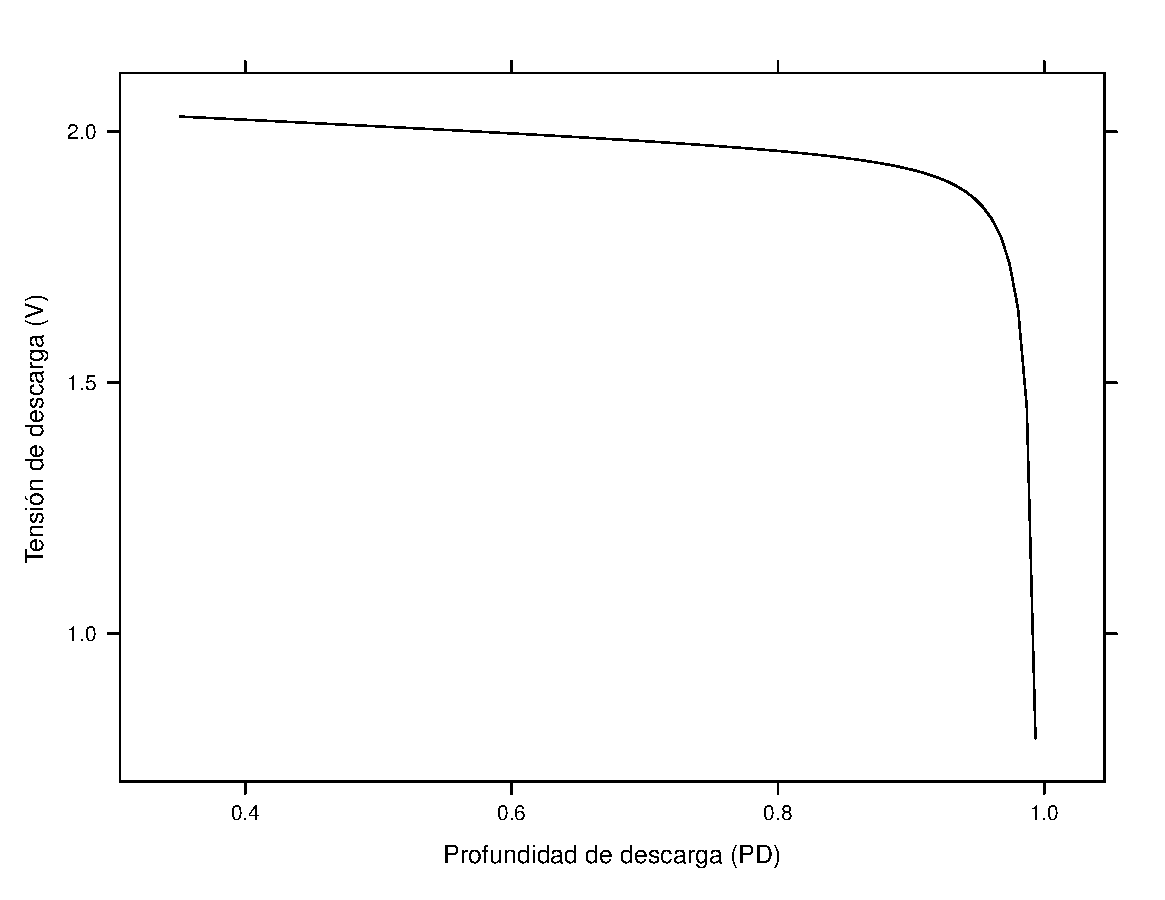
\includegraphics[width=.9\linewidth]{../figs/Bateria_SOCyDescarga.pdf}
\end{center}
\end{frame}

\begin{frame}[label={sec:org9a226ea}]{Evolución de la tensión en un proceso de carga}
\begin{center}
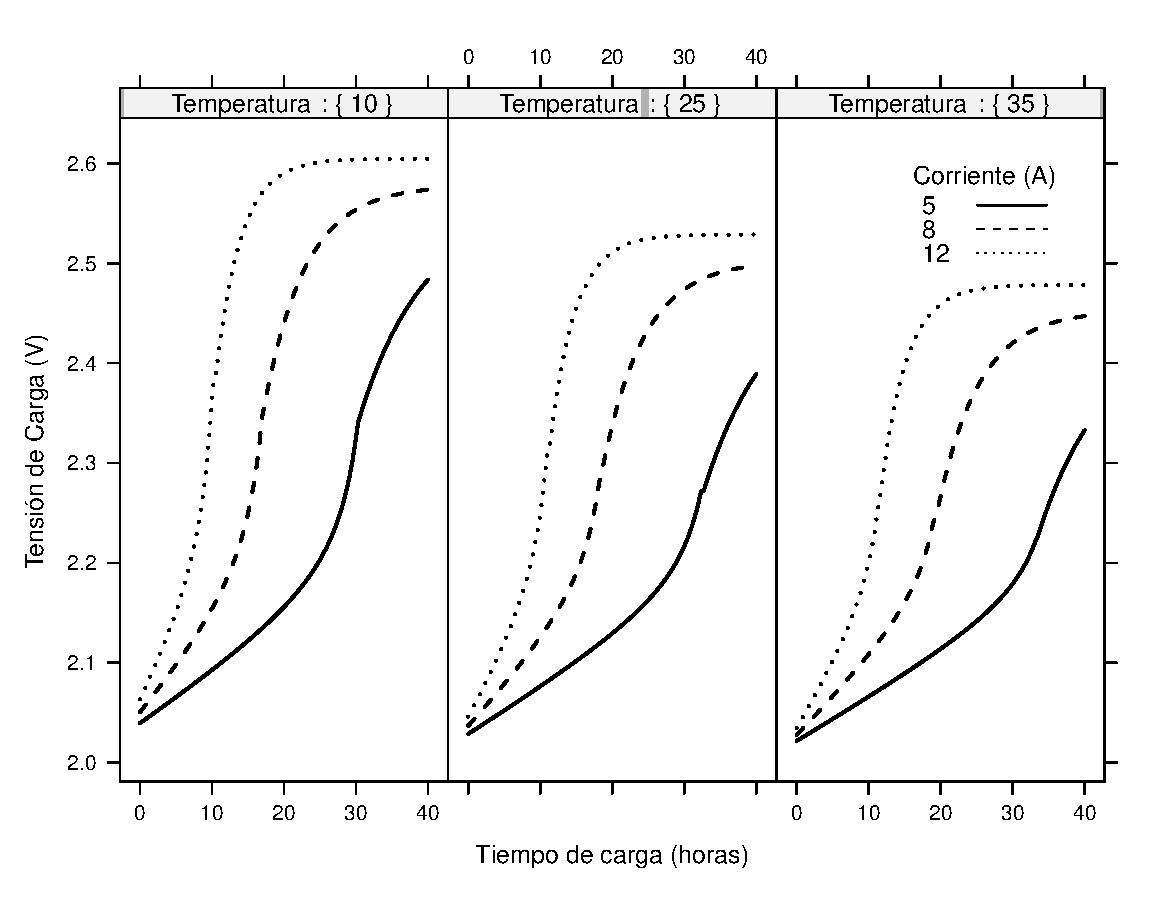
\includegraphics[width=.9\linewidth]{../figs/Bateria_CorrYTemp.pdf}
\end{center}
\end{frame}


\subsection{Efecto de la temperatura}
\label{sec:org23e6115}

\begin{frame}[label={sec:org1e3d113}]{Temperatura baja}
\begin{itemize}
\item El electrolito se hace más viscoso y decrece la movilidad de los iones (aumenta la resistencia eléctrica)

\item \alert{Baja la capacidad} para un regimen de descarga determinado a razón de 1\%/ºC

\item Si el electrolito se congela, no hay movimiento iónico, y por tanto la capacidad es nula. Para evitarlo, \alert{hay que recurrir a densidades altas de electrolito en lugares muy frios}.
\end{itemize}
\end{frame}

\begin{frame}[label={sec:orge5ac5e4}]{Temperatura alta}
\begin{itemize}
\item \alert{Acelera las reacciones, favoreciendo la corrosión}. Por tanto, decrece la vida de la batería.

\item En \alert{climas cálidos}, se debe optar por \alert{bajas concentraciones de electrolito} (que se ve compensada por la mayor movilidad iónica debida a la alta temperatura).

\item \alert{Baja el valor de tensión al que empieza la sobrecarga} debido a que la resistencia interna baja con la temperatura.

\begin{itemize}
\item Hay que corregir el umbral de corte con la temperatura (se puede utilizar la ambiente como referencia)
\end{itemize}
\end{itemize}
\end{frame}

\begin{frame}[label={sec:org69ea7f7}]{Capacidad según el regimen de descarga y la temperatura}
\begin{center}
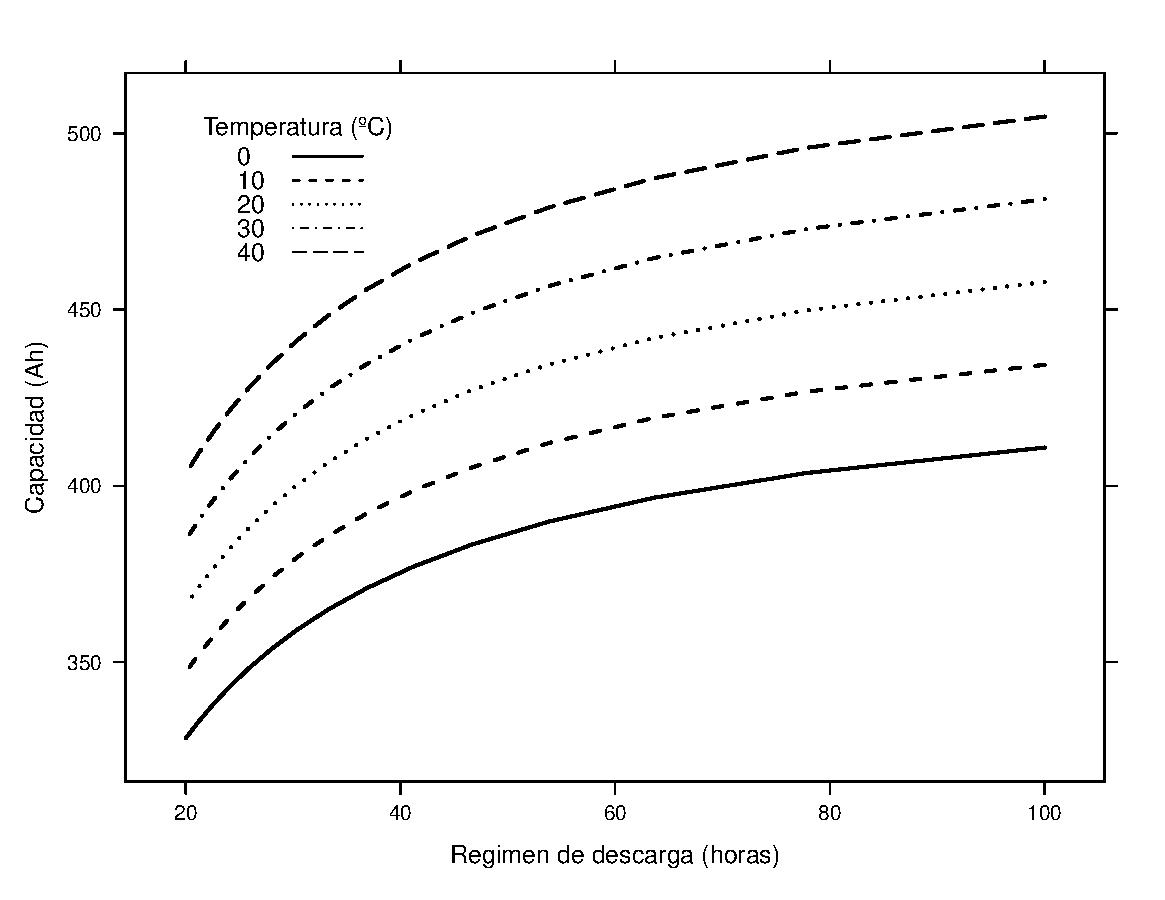
\includegraphics[width=.9\linewidth]{../figs/Bateria_Capacidad.pdf}
\end{center}
\end{frame}

\subsection{Ciclado}
\label{sec:orge4aebc2}
\begin{frame}[label={sec:org86c6871}]{Definición}
\begin{itemize}
\item El ciclado es el \alert{proceso} por el que un acumulador es \alert{continuamente cargado y descargado durante su vida.}

\item Produce \alert{degradación} de la batería por \alert{perdida de material activo} (descargas repetidas) y \alert{estratificación}.
\end{itemize}
\end{frame}

\begin{frame}[label={sec:orgca9e363}]{Resistencia al ciclado}
Los factores que influyen sobre la resistencia del acumulador al ciclado son: 
\begin{itemize}
\item \alert{La profundidad de descarga}: las descargas profundas disminuyen los ciclos de vida de una batería.

\item \alert{El régimen de carga}: cuanto mayor es el régimen de carga y el porcentaje de sobrecarga, menor será la vida alcanzada.

\item \alert{La temperatura}: las temperaturas altas aceleran la corrosión en los electrodos disminuyendo los ciclos de vida.
\end{itemize}
\end{frame}


\subsection{Composición}
\label{sec:org65118d2}

\begin{frame}[label={sec:org8228a0d}]{Composición}
\begin{center}
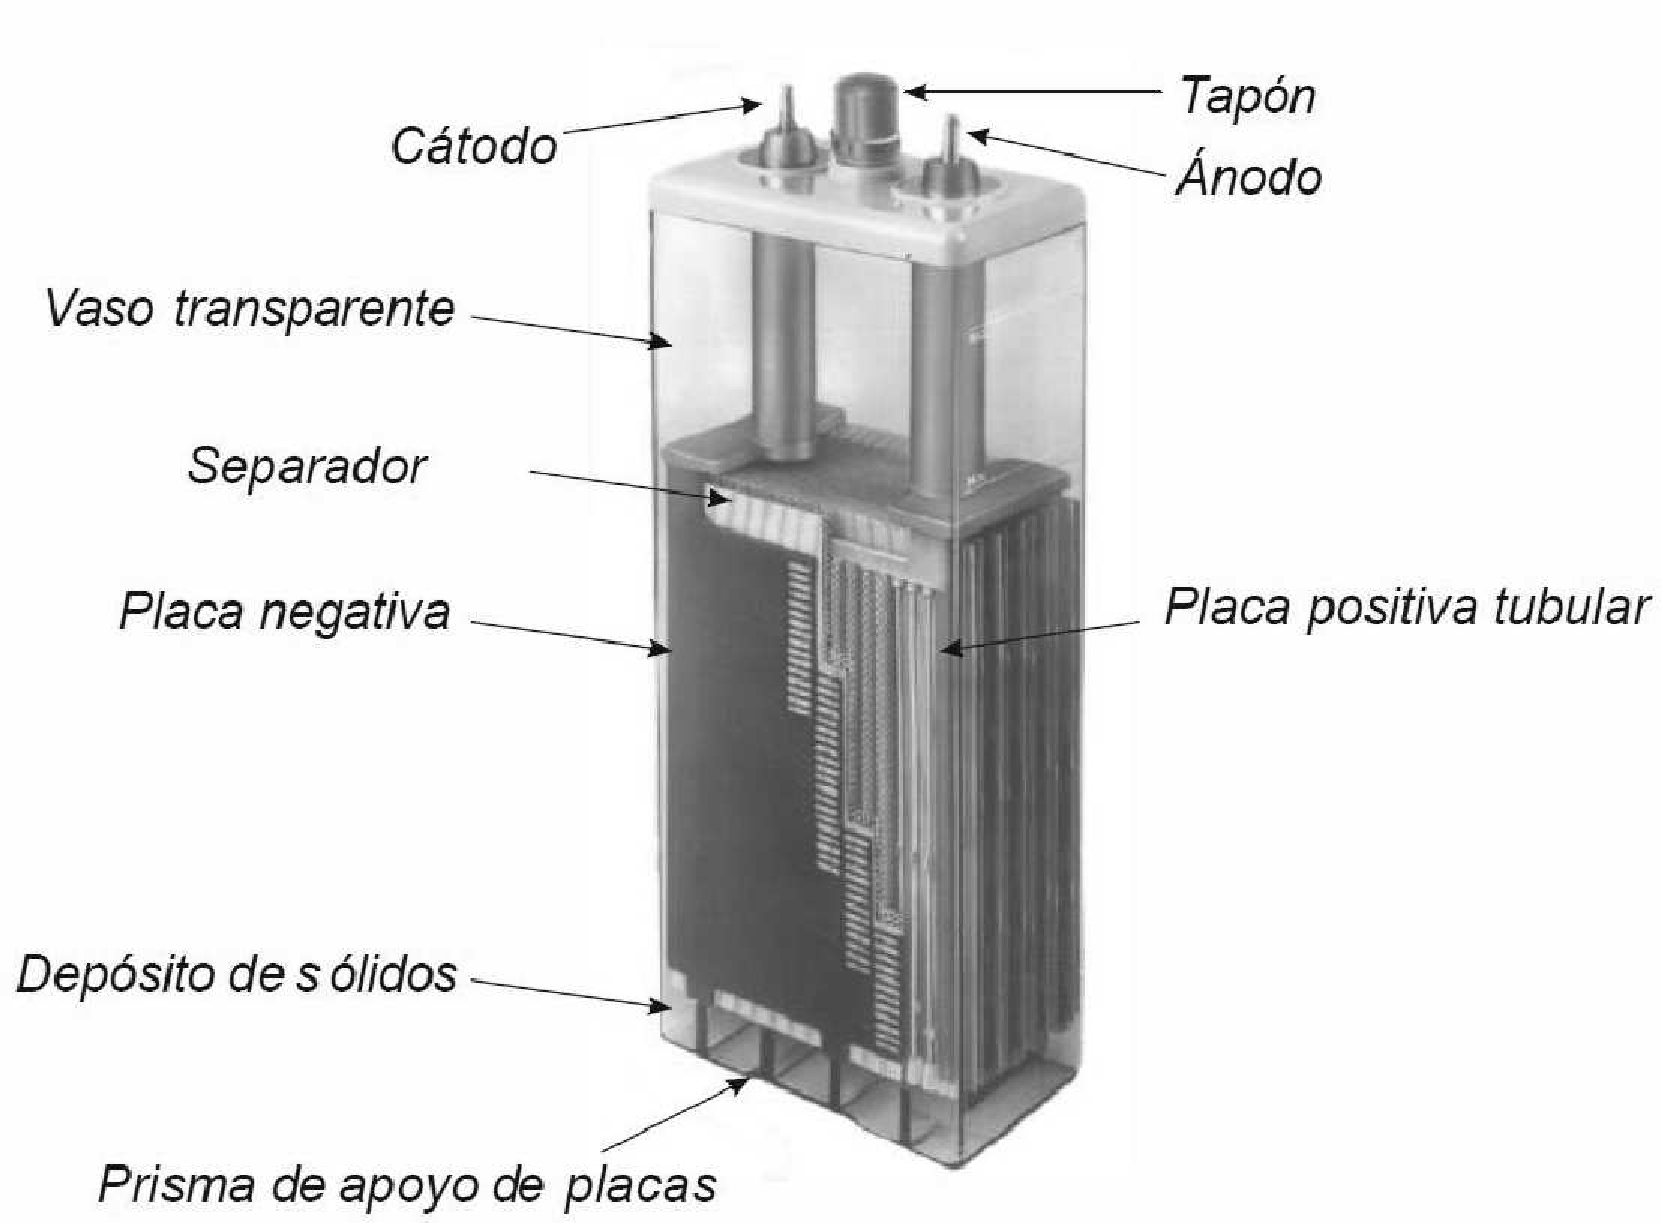
\includegraphics[width=.9\linewidth]{../figs/AcumuladorBN.pdf}
\end{center}
\end{frame}

\begin{frame}[label={sec:org1708039}]{Rejillas}
\begin{itemize}
\item Dan \alert{soporte estructural a los materiales activos}

\item \alert{Conducen la corriente eléctrica} hacia el circuito externo.

\item Están fabricadas en \alert{aleaciones de Plomo}.

\begin{itemize}
\item La \alert{aleación de plomo-antimonio} presenta buen comportamiento en
ciclado y en descarga profunda.
\end{itemize}

\item La \alert{rejilla negativa} es \alert{plana}

\item La \alert{rejilla positiva} puede ser \alert{plana} (operación en flotación) o
\alert{tubular} (operación en ciclado).
\end{itemize}
\end{frame}

\begin{frame}[label={sec:orgeb67269}]{Materiales activos}
\begin{itemize}
\item Los materiales activos participan en las reacciones químicas.
\item Están \alert{adheridos a las rejillas}.
\item Deben ser \alert{porosos} para permitir la penetración del electrolito
\end{itemize}
\end{frame}

\begin{frame}[label={sec:org6112114}]{Electrolito}
\begin{itemize}
\item El \alert{electrolito} participa en la reacción y \alert{realiza el transporte
iónico} para cerrar el ciclo de corriente de las reacciones.

\item Para \alert{reducir la resistencia eléctrica} del electrolito, su \alert{densidad
debe ser alta},

\item Pero \alert{un electrolito de alta densidad es muy agresivo} (produce
corrosión en la rejilla positiva).

\item Los acumuladores estacionarios utilizan densidades más bajas que
los de arranque (altos regímenes de descarga).

\item El electrolito \alert{puede ser líquido} (aireadas) \alert{o inmovilizado}
(selladas).
\end{itemize}
\end{frame}

\begin{frame}[label={sec:org6aada3d}]{Separadores}
\begin{itemize}
\item Los separadores \alert{aislan las placas de diferente polaridad pero
permiten el movimiento iónico a través suyo}.
\item Requisitos:
\begin{itemize}
\item Resistencia mecánica
\item Permeables y porosos.
\item Resistentes a la oxidación
\item Aislantes eléctricos
\item Sin contaminantes
\end{itemize}
\end{itemize}
\end{frame}

\subsection{Tipos de acumuladores}
\label{sec:org74b34c7}

\begin{frame}[label={sec:orgd54c7ab}]{Características generales}
\begin{itemize}
\item Un acumulador incorporado a un SFA debe ser \alert{capaz de funcionar sometido a ciclados diarios y anuales de carga y descarga}, teniendo en cuenta que la carga entregada por el generador depende directamente de la radiación (variable en los períodos intradiario e intraanual).

\item Debido a las posibles fluctuaciones en la carga aportada, es probable que se sucedan \alert{periodos prolongados en carga parcial}.

\item Es habitual que las \alert{descargas sean a baja intensidad con periodos de descarga largos}, típicamente en torno a las 100 horas.
\end{itemize}
\end{frame}

\begin{frame}[label={sec:org969b15f}]{Baterías de arranque}
\begin{itemize}
\item Habitualmente empleadas en automóviles

\item Fácilmente localizables en cualquier mercado local a bajo precio (relativo)

\item Opción frecuentemente empleada en sistemas de electrificación rural de pequeño tamaño

\item Reemplazo de baterías estropeadas

\item Buen comportamiento en descarga de alta intensidad y tienen buen rendimiento de descarga a bajas temperaturas.

\item No son resistentes frente al ciclado
\end{itemize}
\end{frame}

\begin{frame}[label={sec:orge1791cd}]{Baterías de tracción}
\begin{itemize}
\item Empleadas, por ejemplo, en carretillas elevadoras.

\item Resistencia suficiente para soportar un elevado número de ciclos profundos de carga-descarga.

\item Requieren aportación de agua y mantenimiento frecuente.

\item Empleo en SFA sólo cuando exista mantenimiento regular.
\end{itemize}
\end{frame}

\begin{frame}[label={sec:org17d8713}]{Baterías estacionarias}
\begin{itemize}
\item Empleadas en sistemas de alimentación ininterrumpida (UPS) o instalaciones remotas (por ejemplo, radioenlaces).

\item Funcionan en régimen de flotación.

\item Gran reserva de electrolito aunque realizan poco uso de agua.

\item Resistencia a la corrosión y elevada fiabilidad.

\item Opción muy interesante para SFA. Precio más elevado frente a las anteriores opciones.
\end{itemize}
\end{frame}

\begin{frame}[label={sec:org28ab366}]{Elección de batería}
\begin{itemize}
\item Criterios a tener en cuenta:

\begin{itemize}
\item \alert{Requisitos técnicos} (capacidad, tipo de ciclado, etc.)

\item \alert{Coste del sistema}

\item Recursos de \alert{mantenimiento} disponibles durante la vida del sistema,

\item \alert{Disponibilidad de reemplazo} en el mercado local

\item Capacidad de intervención del usuario.
\end{itemize}

\item \alert{Para aplicaciones fotovoltaicas} se recomienda:

\begin{itemize}
\item \alert{Baterías estacionarias aireadas de placa positiva tubular}

\item \alert{Baterías SLI modificadas}: placas más gruesas, mayor cantidad de
electrolito por encima de las placas, con aleación de Pb-Sb en la
rejilla y vaso transparente.
\end{itemize}
\end{itemize}
\end{frame}

\section{Regulador de carga}
\label{sec:orgba11ea8}

\begin{frame}[label={sec:org0793d7b}]{Definición}
Un regulador de carga es un equipo electrónico capaz de \alert{evitar la sobrecarga y la descarga excesiva de un acumulador} desconectando al acumulador del generador o del consumo \alert{cuando se alcanzan determinados estados umbral, generalmente determinados por la tensión en bornes}.
\end{frame}

\begin{frame}[label={sec:orgbfb6463}]{Regulador Serie y paralelo}
\begin{itemize}
\item Regulador Serie
\end{itemize}
\begin{center}
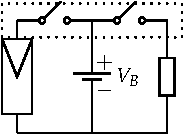
\includegraphics[height=0.3\textheight]{../figs/ReguladorSerie.pdf}
\end{center}

\begin{itemize}
\item Regulador Paralelo
\end{itemize}
\begin{center}
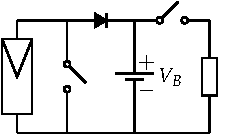
\includegraphics[height=0.3\textheight]{../figs/ReguladorParalelo.pdf}
\end{center}
\end{frame}


\begin{frame}[label={sec:org6b5b458}]{Ciclo de carga}
\begin{center}
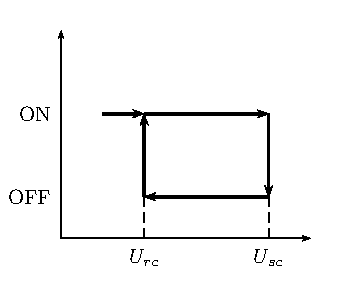
\includegraphics[height=0.5\textheight]{../figs/HisteresisCargaRegulador.pdf}
\end{center}

\begin{itemize}
\item \(U_{sc}\) debe estar en el rango de \(\SI{2.3}{\volt}\) a \(\SI{2.4}{\volt}\) por vaso a \(\SI{25}{\celsius}\).

\item \(U_{rc}\) debe estar en el rango de \(\SI{2.15}{\volt}\) a \(\SI{2.2}{\volt}\) por vaso a \(\SI{25}{\celsius}\).

\item \alert{Deben corregirse por temperatura} a razón de \(\SI{4}{\milli\volt\per\celsius}\) a \(\SI{5}{\milli\volt\per\celsius}\) por vaso.
\end{itemize}
\end{frame}

\begin{frame}[label={sec:orgc888fbb}]{Ciclo de descarga}
\begin{center}
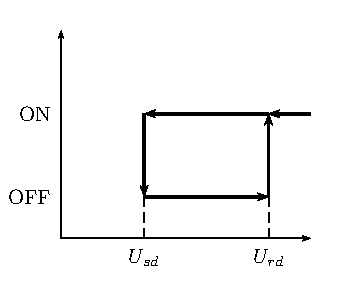
\includegraphics[height=0.5\textheight]{../figs/HisteresisDescargaRegulador.pdf}
\end{center}

Los umbrales deben adaptarse a cada tipo de batería (mediante ensayos, o recomendaciones del fabricante)
\end{frame}

\section{Luminarias}
\label{sec:org6266f10}

\begin{frame}[label={sec:org4c0be50}]{Funcionamiento}
\begin{itemize}
\item Una lámpara fluorescente convencional está formada por un \alert{tubo de descarga con gas a baja presión}, un \alert{recubrimiento de una mezcla de polvos fluorescentes} y \alert{dos electrodos} en los extremos.

\item Un \alert{circuito auxiliar (balasto)} cumple dos funciones principales:

\begin{itemize}
\item \alert{Proporciona la tensión de encendido} necesaria para que fluya corriente por el tubo.

\item \alert{Regula la corriente} que circula por el tubo una vez que se ha producido el encendido para evitar su destrucción.
\end{itemize}
\end{itemize}
\end{frame}

\begin{frame}[label={sec:org3265f0b}]{Degradación}
\begin{itemize}
\item \alert{El proceso de encendido es el que más contribuye a la degradación} de los tubos fluorescentes.
\item Un método alternativo consiste en \alert{precalentar los electrodos} (con un circuito basado en un condensador y en una resistencia) facilitando el paso a la etapa de emisión termoiónica, y acortando el período de encencedido.
\end{itemize}
\end{frame}

\begin{frame}[label={sec:org3eb91fc}]{Fotometría}
\begin{description}
\item[{Flujo}] radiante es la potencia emitida por la fuente luminosa (Unidad: Watio)

\item[{Flujo}] luminoso es la potencia emitida capaz de producir sensación luminosa en el ojo humano (Unidad: Lumen)

\item[{Iluminación}] de una superficie sobre la que incide un flujo luminoso es el ratio entre flujo y superficie (Unidad: lux, \(\si{\lumen\per\watt\squared}\)).

\item[{Eficiencia}] de la luminaria (tubo y balasto) es la relación entre potencia eléctrica consumida por el conjunto y la potencia luminosa producida (Unidad: \(\si{\lumen\per\watt}\)).
\end{description}
\end{frame}

\begin{frame}[label={sec:orgdfbf88a}]{Requisitos}
\begin{itemize}
\item Recomendable eficiencia superior a 50 \(\si{\lumen\per\watt}\)

\begin{itemize}
\item \alert{Debe ser superior a 35 \(\si{\lumen\per\watt}\)}.
\end{itemize}

\item Recomendable resistencia a un mínimo de 10000 ciclos de encendido y apagado

\begin{itemize}
\item \alert{Deberá resistir 5000 ciclos.}
\end{itemize}
\end{itemize}
\end{frame}
\end{document}